\documentclass{article}

\usepackage{tikz}
\usepackage{amsmath}
\usepackage{amssymb}

\newcommand{\myabs}[1]{\vert#1\vert}
\newcommand{\pder}[2]{\frac{\partial#1}{\partial#2}}

\DeclareMathOperator{\iso}{Iso}
\DeclareMathOperator{\fix}{Fix}
\DeclareMathOperator{\tr}{Tr}
\DeclareMathOperator{\vol}{Vol}

\setlength\parindent{0pt}

\begin{document}
\begin{figure}
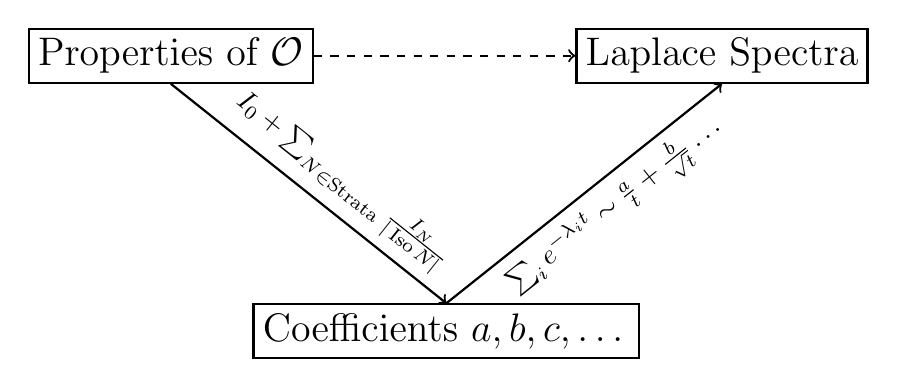
\begin{tikzpicture}[scale = 0.7]
    \node[draw,thick] (O) at (0,5) {\Large{Properties of $\mathcal{O}$}};
    \node[draw,thick] (a) at (5,0) {\Large{Coefficients $a,b,c,\dots$}};
    \node[draw,thick] (L) at (10,5) {\Large{Laplace Spectra}};
    \draw[->,thick] (O.south) -- (a.north) node [midway,sloped,above] (test) {\ \ \ \ $I_0+\sum_{N \in \text{Strata}}\frac{I_N}{\myabs{\iso N}}$}; 
    \draw[->,thick] (a.north) -- (L.south) node [midway,sloped,below]
    (test) {\ \ \ \ $\sum_{i}e^{-\lambda_i t} \sim \frac{a}{t} +
    \frac{b}{\sqrt{t}}\dots$};
    \draw[->,thick,dashed] (O) -- (L);
    \end{tikzpicture}
\end{figure}
\end{document}
